\documentclass[11pt]{article}
% \usepackage[utf8]{inputenc}
\usepackage{deauthor,times,graphicx}
\usepackage{enumitem}
% \setlist{nolistsep,leftmargin=*}

%%%% macros.tex

%\usepackage{anysize}
%\usepackage{geometry}
%\geometry{top=1in, left=1in, right=1in, bottom=1in,footskip=.25in}
%\marginsize{1in}{0.8in}{1in}{1in}%tblr
%\usepackage[showframe,bottom=0.2in,footskip=.25in]{geometry}
%\usepackage[left=1in, right=1in, top=1in]{geometry}
%\newcommand{\cmt}[2]{\textcolor{dkmag}{[#1: #2]}}
%\newcommand{\personname}[1]{\cmt{Personname}{#1}}
%\newcommand{\standout}[1]{\textit{\textcolor{dkmag}{#1}}}
%usepackage[T1]{fontenc}
%\usepackage{fontspec}
%\setmainfont[Scale=0.85, Ligatures={Required,Common,Contextual,TeX}]{TeX Gyre Schola} % Incredible font inside latex

%
%\usepackage{fancyhdr}
%\usepackage{fullpage} %, hyperref}
%\usepackage{amssymb, amsmath, enumitem, titling, hyperref}
%\usepackage[standard]{ntheorem}
%%\usepackage[sort&compress]{natbib}
%\usepackage[top=0.65in, bottom=1.2in, left=0.95in, right=0.95in]{geometry}
% %\ifthenelse{\value{page}=1}
%          %{\setlength\headheight{40pt}}
%          %{\setlength\headheight{0pt}}
%
%\usepackage[backend=bibtex,sorting=anyt, maxnames=7, firstinits=true]{biblatex} %hyperref=true,
%\renewcommand*{\bibfont}{\footnotesize}
%\bibliography{bib_rs}
%%\renewcommand{\baselinestretch}{0.9}
\usepackage{multirow}
\usepackage{float}
\usepackage{caption}
%\usepackage{subfloat}
%\usepackage{float}
\usepackage{amsmath}
\usepackage{graphicx, multicol, latexsym, amsmath, amssymb}
\usepackage{blindtext}
\usepackage{caption}
\def\sharedaffiliation{%
\end{tabular}
\begin{tabular}{c}}
\newcommand{\vset}[1]{\mathbf{#1}}
%\usepackage{amsthm}
%
%\theoremstyle{definition}
%\newtheorem{definition}{Definition}[section]
% end Spencer

\newcommand{\reva}[1]{{ { { #1}}}}
\newcommand{\revb}[1]{{{ { #1}}}}
\newcommand{\revc}[1]{{{{ #1}}}}
\newcommand{\revd}[1]{{{{ #1}}}}
\newcommand{\reve}[1]{{{ { #1}}}}
%\newcommand{\revf}[1]{{{\color{red} {#1}}}}




\newcommand{\mypm}{\mathbin{\tikz [x=1.4ex,y=1.4ex,line width=.1ex] \draw (0.0,0) -- (1.0,0) (0.5,0.08) -- (0.5,0.92) (0.0,0.5) -- (1.0,0.5);}}%


\newcommand{\qii}{\delta}

\newcommand{\createcontingencytable}[4]{ %
	% #1=table name
	% #2=first column name
	% #3=new row sum name
	% #4=new column sum name
	\pgfplotstablecreatecol[
	create col/assign/.code={% In each row ...
		\def\rowsum{0}
		\pgfmathtruncatemacro\maxcolindex{\pgfplotstablecols-1}
		% ... loop over all columns, summing up the elements
		\pgfplotsforeachungrouped \col in {1,...,\maxcolindex}{
			\pgfmathsetmacro\rowsum{\rowsum+\thisrowno{\col}}
		}
		\pgfkeyslet{/pgfplots/table/create col/next content}\rowsum
	}
	]{#3}{#1}%
	%
	% Transpose the table, so we can repeat the summation step for the columns
	\pgfplotstabletranspose[colnames from={#2},input colnames to={#2}]{\intermediatetable}{#1}
	%
	% Sums for each column
	\pgfplotstablecreatecol[
	create col/assign/.code={%
		\def\colsum{0}
		\pgfmathtruncatemacro\maxcolindex{\pgfplotstablecols-1}
		\pgfplotsforeachungrouped \col in {1,...,\maxcolindex}{
			\pgfmathsetmacro\colsum{\colsum+\thisrowno{\col}}
		}
		\pgfkeyslet{/pgfplots/table/create col/next content}\colsum
	}
	]{#4}\intermediatetable
	%
	% Transpose back to the original form
	\pgfplotstabletranspose[colnames from=#2, input colnames to=#2]{\contingencytable}{\intermediatetable}
}
%

% \PassOptionsToPackage{hyphens}{url}\usepackage{hyperref}
\newcommand{\inp}{{{\mb X }}}
\newcommand{\cm}{{{\mb M }}}
\newcommand{\acm}{{{\mb M_{\mc A} }}}
\newcommand{\cg}{ G}
\newcommand{\acg}{ G_{\mb M_{\mc A}} }

\newcommand{\nipsadult}{{{Binned Adult}}}
\newcommand{\nipscompas}{{{Binned COMPAS}}}
\usepackage{booktabs,siunitx}
% \DeclareMathOperator*{\argmax}{argmax}
% \DeclareMathOperator*{\argmin}{argmin}
\newcommand{\fge}{{\bf {FGE}}}
\newcommand{\scmit}{{\bf {SNMIT}}}
\newcommand{\cmit}{{\bf {MIT}}}
\newcommand{\icmit}{{\bf {FNMIT}}}
\newcommand{\iscmit}{{\bf {FMIT}}}
\newcommand{\hcmit}{{\bf {HyMIT}}}
\newcommand{\ogsal}{{\bf {OGS}}}
\newcommand{\gsal}{{\bf {GS}}}
\newcommand{\pdal}{{\bf {CD}}}
\newcommand{\delay}{{\tt \textsc{Flight Delay}}}
\newcommand{\ate}{{\tt \textsc{ATE}}}
\newcommand{\nde}{{\tt \textsc{NDE}}}
\newcommand{\nie}{{\tt \textsc{NIE}}}
\newcommand{\E}{{\tt \mathbb{E}}}
\newcommand{\pr}{{\tt \mathrm{Pr}}}
\newcommand{\hsys}{{\textsc{HypDB}}}
\newcommand{\sys}{{\textsc{Capuchin}}}
\newcommand{\dal}{{{SGS}}}
\newcommand{\bigCI}{\mathrel{\text{\scalebox{1.07}{$\perp\mkern-10mu\perp$}}}}
\newcommand{\nbigCI}{\cancel{\mathrel{\text{\scalebox{1.07}{$\perp\mkern-10mu\perp$}}}}}
\newcommand{\rred}[1]{\textcolor{red}{#1}}
\newcommand{\mc}[1]{\mathcal{#1}}
\newcommand{\ind}[0]{\textrm{Indep}}
\newcommand{\ignore}[1]{}
\newcommand{\comlb}[1]{{\vspace{2mm}\noindent \rred{\bf COMM(Dan):}}~ #1 \hfill {\bf    END.}\\}
\newcommand{\combabak}[1]{{\vspace{4mm}\noindent \bf  COMM(Babak):}~ {\em \rred{#1}}\hfill {\bf END.}\\}



\newcommand*{\rom}[1]{\expandafter\@slowromancap\romannumeral #1@}

\newcommand{\dan}[1]{{{\color{red} {\bf\underline{Dan}}: [{#1}]}}}
\newcommand{\babak}[1]{{\texttt{\color{red} Babak: [{#1}]}}}
\newcommand{\bill}[1]{{\texttt{\color{olive} Bill: [{#1}]}}}
\newcommand{\luke}[1]{{\texttt{\color{blue} Luke: [{#1}]}}}
\newcommand{\johannes}[1]{{\texttt{\color{blue} Johannes: [{#1}]}}}
\newcommand{\red}[1]{{\textbf {{\color{red} [{#1}]}}}}
\newcommand{\scream}[1]{{\texttt{\color{red}{\textbf{[{#1}]}}}}}

\newcommand{\LOGSPACE}{{\scriptsize $  \mathrm{LOGSPACE}$}}
\newcommand{\NLOGSPACE}{{\scriptsize $  \mathrm{NLOGSPACE}$}}
\newcommand{\PTIME}{{\scriptsize $  \mathrm{PTIME}$ }}
\newcommand{\nindep}{\mbox{$\not\!\perp\!\!\!\perp$}}
\newcommand{\indep}{\mbox{$\perp\!\!\!\perp$}}





\newcommand{\tr}{1} %{\mathtt{t}}
\newcommand{\cn}{0} %{\mathtt{c}}

%infotheo
\newcommand{\rep}{D'}
\newcommand{\icq}{Q_\varphi}
\newcommand{\hb}{D^*}


\newcommand{\satt}{\mathbf{a}}
\newcommand{\att}{\mathbf{A}}
\newcommand{\sx}{\mathbf{x}}
\newcommand{\bx}{\mathbf{X}}
\newcommand{\pn}{\textmd{N}}
\newcommand{\ent}{{\mathcal{H}}}
\newcommand{\minf}{{{I}}}
\newcommand\mvd{\twoheadrightarrow}
\newcommand{\amvd}{\twoheadrightarrow_\alpha}
\newcommand{\fd}{\rightarrow}
\newcommand{\afd}{\rightarrow_\alpha}
\newcommand{\bfd}{\rightarrow_\beta}
\newcommand{\abfd}{\rightarrow_{\alpha+\beta}}
\newcommand{\A}{\texttt{A}}
\newcommand{\K}{\texttt{K}}
\newcommand{\deletelater}[1]{{\textbf {{\color{green} [{#1}]}}}}
\newcommand{\intervrel}{\texttt{intervened-relation}}

\newcommand{\annot}{\texttt{annot}}
\newcommand{\supp}{\texttt{supp}}
\newcommand{\sch}{{\mathcal{S}}}
\newcommand{\rel}{{\mathcal{R}}}
%\newcommand{\interv}{{\Gamma}}
\newcommand{\real}{{\mathbb{R}}}
\newcommand{\nat}{{\mathbb{N}}}
\newcommand{\explattr}{{\{E\}}}
%\newcommand{\change}{{\Delta}}
\newcommand{\bool}{{\textit{b}}}


\newcommand{\AP}{\texttt{AP}}
\newcommand{\highval}{\texttt{high}}
\newcommand{\midval}{\texttt{mid}}
\newcommand{\lowval}{\texttt{low}}
\newcommand{\aplow}{\texttt{poor}}
\newcommand{\aphigh}{\texttt{good}}
\newcommand{\dbnull}{\texttt{null}}
\newcommand{\relset}{\mathcal{R}}
\newcommand{\reltop}{{\mathcal{R}}_{top}}
\newcommand{\relbot}{{\mathcal{R}}_{bot}}
\newcommand{\attrset}{\mathcal{A}}
\newcommand{\attrtop}[1]{{\mathcal{A}}_{{top}, {#1}}}
\newcommand{\attrbot}{{\mathcal{A}}_{bot}}
%\newcommand{\featureset}{\mathcal{B}}
\newcommand{\wcl}{\mathscr{C}(\mb{C})}
\newcommand{\rwq}{{ {\mc{Q}_{rw}}}}
\newcommand{\db}{{D}}
\newcommand{\dbdom}{\mathbf{DB}}
\newcommand{\intervadditive}{{intervention-additive}}
\newcommand{\val}{{v}}
\newcommand{\valorig}{{u}}
%\newcommand{\dbdom}{\mathcal{D}}
\newcommand{\inputclass}{\mathcal{C}}
%\newcommand{\intervene}{\mathcal{I}}
%\newcommand{\tbaff}{{\tt{T_{Aff}}}}
%\newcommand{\attaff}{{\tt{A_{Aff}}}}
\newcommand{\univ}{{{U}}}
\newcommand{\pk}{{\mathtt{pk}}}
\newcommand{\fk}{{\mathtt{fk}}}
\newcommand{\expl}{{\phi}}
%\newcommand{\pk}{{\tt \mathtt{\pk}}}
\newcommand{\sign}{{\tt \mathtt{sign}}}
%\newcommand{\expldom}{{\Phi}}

\newcommand{\select}{\tt {\textsc{Select}}}
\newcommand{\where}{{\tt \textsc{Where}}}
\newcommand{\with}{{\tt \textsc{With}}}
\newcommand{\distinct}{{\tt \textsc{distinct}}}
\newcommand{\groupby}{{\tt \textsc{Group By}}}
\newcommand{\from}{{\tt \textsc{From}}}
\newcommand{\ct}{{\tt \textsc{Count}}}
\newcommand{\create}{{\tt \textsc{Create}}}
\newcommand{\explanation}{{\tt \textsc{Explanation}}}
%\newcommand{\Pr}{{\tt {Pr}}}
\newcommand{\on}{{\tt \textsc{On}}}
\newcommand{\sqlwith}{{\tt \textsc{With}}}
\newcommand{\as}{{\tt \textsc{as}}}
\newcommand{\cascade}{{\tt \textsc{Cascade}}}
\newcommand{\sqland}{{\tt \textsc{And}}}
\newcommand{\sqlin}{{\tt \textsc{In}}}
\newcommand{\true}{{\tt true}}
\newcommand{\false}{{\tt false}}
\newcommand{\inmath}[1]{{\mathtt {#1}}}

\newcommand{\RNum}[1]{\uppercase\expandafter{\romannumeral #1\relax}}
\newcommand{\ie}{{\em i.e.}} %\xspace}
\newcommand{\eg}{{\em e.g.}} %\xspace}
\newcommand{\etal}{{et al.}} %\xspace}
\newcommand{\aka}{{\em a.k.a.}\xspace}
\newcommand{\algorithmicbreak}{\textbf{Break}}
\newcommand{\backwd}{\mathcal{B}}
\newcommand{\mbl}{{\bf B}}
\newcommand{\mmb}{{\bf MB}}
\newcommand{\emb}{{ \bf MB}_\epsilon}
\newcommand{\embl}{{\bf B}_\epsilon}
\newcommand{\emmb}{{\bf IB}_{(\epsilon,\beta)}}
\newcounter{enumQues}
\newcommand{\mf}[1]{\mathrm{\mathfrak{#1}}}
\newcommand{\mb}[1]{{\mathbf{#1}}}
% \newtheorem{defn}{Definition}[section]
% \newtheorem{rem}[defn]{Remark}
% \newtheorem{conj}[defn]{Conjecture}
% \newtheorem{prop}[defn]{Proposition}
% \newtheorem{obs}[defn]{Observation}
% \newtheorem{assumption}[defn]{Assumption}
\newcommand{\proj}[1]{{\Pi}}
\newcommand{\sel}[1]{{\sigma}}

\newcommand{\un}[1]{{\underline{#1}}}
\newcommand{\ov}[1]{{\overline{#1}}}
\newcommand{\cut}[1]{}
\newcommand{\eat}[1]{}

\newcommand{\causalframework}{interventional fairness}
\newcommand{\metric}{interventional discrimination}
\newcommand{\fairalgorithm}{interventional fairness}

\newcommand{\defeq}{\stackrel{\text{def}}{=}}

\newcommand{\fairapp}{fairness application~}

\newcommand\blfootnote[1]{%
  \begingroup
  \renewcommand\thefootnote{}\footnote{#1}%
  \addtocounter{footnote}{-1}%
  \endgroup
}




%%%%%%%%%%%



\begin{document}
\title{Fairness in Practice: A Survey on Equity in Urban Mobility} 


\author{An Yan, \  Bill Howe \\
University of Washington\\
\{yanan15,billhowe\}@uw.edu}

\maketitle
\blfootnote{This work is supported by the National Science Foundation under grant NSF BIGDATA-1740996.}

\section{Introduction}
More than 54 percent of the world's population lives in urban areas \cite{zhang2017regions}. Predicting dynamic urban activities such as energy consumption, air pollution, public safety, and traffic flows has become a fundamental task for improving the quality of human life. Urban mobility is closely intertwined with these problems, and is therefore a major determinant of quality of life \cite{shafrin2017association}, crucial to employment opportunities and access to resources such as education and health care \cite{chan2016screening}. %Prediction tasks for urban mobility include transport resource demand prediction, travel time prediction, traffic flows prediction, ride-hailing waiting time estimation, and behavior analysis for autonmous vehicles. 

Evidence suggests that residents of low-income and minority neighborhoods are concentrated away from economic opportunity and public resources \cite{wang2018urban}. Injustice of transportation services experienced by these residents further reinforces social exclusion as the availability and quality of transportation impact a person’s access to opportunities \cite{litman2018evaluating, shaheen2017travel, palmateer2017justice, ricciardi2015exploring}. For example, one study revealed that living in neighborhoods with longer commute times is associated with lower employment rates of younger generations \cite{chetty2016childhood}. As a result, transportation equity issues have motivated government agencies to develop extensive multimodal transportation networks\cite{shaheen2017travel}. 

\textit{New mobility }is about emerging transportation modes, including but not limited to car-sharing, bike-sharing, and ride-hailing or Transportation Network Companies (TNCs) \cite{goldman2006sustainable}. New mobility services provide technology-based, on-demand, and affordable alternatives to traditional means. These services offer a chance to address persistent equity issues in transportation. However, new mobility services also bring new equity concerns. For example, people without internet service, smart phones, or credit cards are not able to get access to the services. Moreover, studies show that algorithms or human beings that distribute app-based mobility services may discriminate against people of color \cite{ge2016racial}. 
%Although a line of equity research has been developed to  focus on new mobility systems, the equity implications of them are not well understood. 

This paper reviews the methods and findings of mobility equity studies, with a focus on new mobility. The paper is structured as follows: Section \ref{sec:headings} presents the background of transportation equity. Section 3 summarizes the main findings from current equity studies for mobility systems, with a brief discussion on future research. Section 4 reviews the commonly used methods for evaluating the equity of mobility service provision and usage and considers strengths and weaknesses.  Section 5 discusses the relationship between the transportation equity community and the fairness in machine learning community. Section 6 concludes the paper. 


% Modern scientific methods including hypothesis testing, computer simulation, process-based models, and machine learning have witnessed success in tacking urban challenges in the past decades [cite].  Recent advances of deep learning, and the growing availability of urban data offer exciting challenges opportunities for extending our capability to model the spatio-temporal dynamics of urban events from data with exceptional accuracy. Among the many aspects of urban events, this paper focuses on mobility and reviews the state of the art deep learning methods for forecasting urban mobility events. 

% Urban mobility, an important aspect of urban  is about how people move around the city using common transport means such as walking, cycling, public transport, car, or motorcycle [Vasconcellos, 2018]. 

% New mobility is an emerging transportation system currently features car-sharing, ride-hailing, and bike-sharing. It is technology-enabled, seamless, and on-demand. 

% Examples of prediction tasks for new mobility include bike / ride-hailing demand prediction, ride-hailing waiting time estimation, and driving behavior analysis for automatic driving cars. 


\section{Equity in Mobility Systems: Background}
\label{sec:headings}

Automated decision systems powered by machine learning and big data have been widely employed in many applications including credit scoring, criminal justice, online advertising, employment, etc \cite{zliobaite2015survey,petrasic2017algorithms, miller2015algorithms, rudin2013predictive}. These systems have been hailed as efficient, objective, and accurate alternatives to human decision makers \cite{barocas2017fairness}. However, increasing evidence has shown that data-driven systems contain biases. For example, Google’s image recognition system wrongly identified black users as gorillas \cite{guynn2015google}. Amazon’s same-day delivery services excluded predominantly black neighborhoods in many cities to a varying degree \cite{ingold2016amazon}. 

Even if the algorithms themselves are well-intentioned, they can replicate and amplify human biases encoded in the data, thus resulting in unequal distribution of impacts across different demographic groups \cite{zliobaite2015survey, lepri2017tyranny, barocas2016big}. This effect is due to machine learning algorithms seeking to fit the training data as closely as possible to make accurate predictions. The process of learning also “accurately” captures historical signals of discrimination. In 2017, Caliskan et al. \cite{caliskan2017semantics} found that an influential language corpus \cite{pennington2014glove} generated by machine learning algorithms accurately reproduced historic biases. The corpus reflects societal stereotypes such as female names are more associated with family while male names are more associated with career. Not only do algorithms pick up discrimination in data, they also magnify them \cite{chouldechova2018frontiers}. This effect is often due to the underrepresentation of minority groups in training data, leading to higher error rates for the minorities. One study \cite{lum2016predict} revealed that a widely-used predictive policing tool, PredPol, would reinforce the bias in the police-recorded, resulting in disproportionate policing of minority communities. 

The heightened concerns about automated decision systems concentrate not only on discrimination, but also on a range of related issues, including transparency, privacy, and accountability \cite{young2019beyond}. These issues often intertwine and conflict with one another in practice. In the context of automatic decision systems, transparency is about the openness and understandability of data and models and accountability is about being responsible for the decisions \cite{lepri2018fair}. Transparency is a critical prerequisite for accountability. In the absence of concrete evidence of intentional discrimination, it is difficult to hold an individual or organization accountable for biased decisions. 

In practice, transparency for automatic decision systems is not easily achievable. Burrell \cite{burrell2016machine} summarized three types of barriers to transparency: 1) intrinsic opacity, where some algorithms such as deep learning models are difficult to understand and interpret; 2) illiterate opacity, which says the general public may lack the expertise to understand the algorithms; and 3) intentional opacity, which is often resulted from intellectual property protection of the algorithm developers. 
%In the Amazon same-day delivery case, white residents were more than twice as likely to live in service areas than black residents in several cities \cite{ingold2016amazon}. The demographic disparities are striking, but we do not have evidence to show that race is part of Amazon’s decision making, because the decision making process is not transparent. Companies like Amazon rarely disclose key technical information for fear of exposing trade secrets and losing competitive advantages. It is thus impossible to further pursue this case to find out the causes of discrimination \cite{diakopoulos2016accountability}.

\subsection{Definitions of transportation equity}
Equity in the context of mobility has been studied independently since well before the recent interest in generalized fairness methods for machine learning.  These efforts suggest that domain-specific and context-sensitive approaches should be incorporated into any fairness-aware ML system.  Equity for mobility is the fair distribution of transportation costs and benefits, among current (and future) members of society \cite{litman2018evaluating}. 

There are mainly two perspectives from which to examine equity: horizontal equity and vertical equity. \textit{Horizontal equity} (also called fairness and egalitarianism) is concerned with providing equal resources to individual or groups considered equal in ability and need, which means the public policies avoid favoring one individual or group over another. Horizontal equity suggests that those who pay more should receive superior services. 

\textit{Vertical equity} (also referred to as social justice, environmental justice, and social inclusion) is concerned with allocating resources to individuals or groups that differ in income, social class, mobility need, or ability.  It advocates that public policies favor disadvantaged groups by providing discounts or special services, therefore compensating for overall inequities. One way to evaluate vertical equity is \textit{equity of opportunity}, meaning that disadvantaged groups should have adequate access to transportation resources. Equity of opportunity is usually measured by access to services. In contrast, “\textit{equity of outcome}” is usually measured by the actual usage of the systems across groups. There is a general agreement about the goal of equity of opportunity, but less agreement about equity of outcome \cite{litman2018evaluating, delbosc2011using,lucas2016method}. 

There are other ways to define transportation equity. Social equity indicates the differences between socioeconomic groups. Spatial equity refers to the differences in transport services among geographic regions \cite{feng2014trade}. These different definitions often overlap or conflict with each other. For example, horizontal equity requires the users to pay for what they get, whereas vertical equity prioritizes the needs of disadvantaged groups such as the low-income or ethnic minorities in the form of discounts \cite{thomopoulos2009incorporating}.

% \subsubsection{Relationship to fairness notions in machine learning community}
% In examining the fairness (equity) definitions from transportation community and machine learning community, I observe that a natural mapping between them can be established, though further effort is needed to create a consistent mapping between concepts in one domain to the other. \textit{Horizontal equity} echoes the spirit of \textit{individual fairness} (similar people should be treated similarly). \textit{Vertical equity} roughly corresponds to \textit{group fairness} (sensitive attributes should be independent from outcomes). This is true in cities where there is an uneven distribution of transport supply across different socioeconomic groups. Vertical equity encourages compensating for such inequalities by policies favoring disadvantaged groups. This aligns with group fairness that the level of transportation supply in a city should be the same across different groups. Vertical equity and group fairness are only "roughly" related because by definition, group fairness stresses "independence" between sensitive attributes and outcome, whereas vertical equity does not.   

\subsection{Evaluation of mobility equity}

Mobility equity research addresses a wide range of issues, including, for example, economic studies on how transportation is subsidized and taxed, and operational studies on how negative impacts of transportation systems are distributed among different groups \cite{shaheen2017travel}. Litman \cite{litman2018evaluating} proposed four variables to consider when performing any equity evaluation.
\begin{itemize}
\item Type of equity: horizontal equity or vertical equity
\item Impact (costs and benefits) categories: public facilities and services, user costs and benefits (e.g., taxes and fares), service quality (e.g., public transportation service quality including frequency, speed, safety, reliability, comfort, etc.), external impacts (e.g., air pollution), economic impacts (e.g., access to employment), and regulation and enforcement (e.g., parking regulations)
\item Measurement unit: per capita, per unit of travel (e.g., per trip), or per dollar. 
\item Categorization of people: demographics (e.g., age, household type, race), income class, ability, location, mode (e.g., pedestrians, public transit), industry (e.g., freight, public transit), and trip type (e.g., commutes)
\end{itemize}

This paper focuses on the equity of new mobility systems service provision and usage across different social-economic, demographic, or geographic groups. 


\section{Findings from Equity Research in Mobility Systems}
\label{sec:others}
We describe findings in the literature across 1) public transportation, and 2) new mobility services.

\paragraph{Public transportation}

Transportation equity has long been a major concern of governmental agencies, researchers, and the general public \cite{litman2018evaluating, shaheen2017travel, palmateer2017justice}. Despite the tremendous investment in transportation system development and progress in transportation equity research, there are still many long-standing equity issues resulted from unequal distributions of transport resources across different socioeconomic groups and spatial regions \cite{raphael2002car, bullard2003addressing, ricciardi2015exploring, el2016cost}. A number of studies have found out that an uneven urban development has resulted in a lack of public transport supply for disadvantaged groups.  For example, Vasconcellos \cite{vasconcellos2018urban} pointed out in Brazil, road systems are developed in a radial pattern. Low-income residents usually settled in fringes of the city with irregular pavements or hilly areas that are subject to landslides. The urban centers with good public services are mostly occupied by the high-income people.  Similarly, Ricciardi \cite{ricciardi2015exploring} found that there is an unequal spatial distribution of public transport resources in two Australian cities. Their analysis showed that 70\% of Perth’s population shares one third of the public transit supply. Moreover, three socially disadvantaged groups --– the elderly, low-income, and no-car households have less access to public transport services compared to the overall population. Some studies also showed that the economic burden and negative climate impacts of transportation systems is disproportionately imposed on disadvantaged people \cite{bullard2003addressing, feng2014trade, cohen2017framework}. In recognizing these issues, many cities now have incorporated social equity into urban transportation planning. However, one study found that social equity goals are often not translated into clear and actionable items and there is a lack of appropriate methods for assessing their achievements \cite{manaugh2015integrating, litman2018evaluating}. Current literature on equity in public transport suggests that disadvantaged groups as a whole experience inequitable access to public transport services but suffer from significant negative impacts from the transportation systems. 
%Further development of transportation systems and policies are needed to overcome these issues. 

\subsection{New mobility}
\paragraph{Bikeshare} A number of researchers have studied equity in bikeshare systems. Several studies found that bikeshare stations were typically located in urban centers with high population density \cite{ogilvie2012inequalities, meng2018evaluation}, and there was a lack of stations in low-income areas. In an assessment of bikeshare systems in seven US cities, Ursaki et al. found significant differences in the race, education level, and income of population inside and outside bike share service areas in four cities \cite{ursaki2015quantifying}. Other studies also indicated that in North America, advantaged groups tend to have more access to docked bikeshare than disadvantaged groups \cite{smith2015exploring}.  Recently, free-floating (dockless) bike share systems have been introduced in several major cities in China and the United States \cite{li2018free, mooney2019freedom, xu2018station}. Free-floating bikeshare systems may have different equity landscape from docked systems. There are no stations in the city, therefore there are no fixed service areas. In this way, access to bikes are transient and largely dependent on the placement of individual bikes, which is driven by user demand and companies’ bike rebalancing strategies. As free-floating bikeshare systems are fairly new, the impact on equity are unclear. In examining access equity of dockless bikes in Seattle, Mooney et al. found out that more college-educated and higher-income residents have access to more bikes. They also found out that bike demand is highly correlated with rebalancing destinations \cite{mooney2019freedom}, suggesting that the companies themselves are accountable for equity issues that arise. 

Equal access to bikeshare does not imply equity of actual usage. Several studies found inequalities in the usage of bikeshare systems \cite{daddio2012maximizing, rixey2013station}. For example, Daddio et al. \cite{daddio2012maximizing} found a negative association between station-level usage with non-white population in Washington, D.C. The disparities in use partially stem from the inequalities of access, but there are many other factors that inhibit bikeshare use among disadvantaged groups. McNeil et al. found out that the biggest barrier to bikeshare is traffic safety, regardless of race or income~\cite{mcneil2017breaking}. Lower-income people of color have more concerns about costs of membership and more misconceptions about bikeshare than higher-income white people. Another study \cite{kretman2011bringing} found that credit card requirement, lack of computer access, annual subscription fee, and lack of bike lanes etc. are reported by low-income residents as barriers to bikeshare. Shaheen et al. \cite{shaheen2017travel} identified five types of barriers to use bikeshare including spatial, temporal, economic, physiological, and social barriers, and provided policy recommendations. Overall, current literature suggests that disparities exist in the access and use of bikeshare systems. 

\paragraph{Ride-hailing}
\looseness-1
Ride-hailing can potentially redefine car access, mitigating the mobility divide resulted from car ownership \cite{brown2018ridehail}. But the equity of ride-hailing services remains unclear. Several studies found that the service quality in terms of waiting times is not necessarily associated with the average income or minority fraction of pickup locations \cite{hughes2016transportation, wang2018spatial}. A recent study \cite{brown2018ridehail} found that users in low-income neighborhoods actually use Lyft more frequently than users in high-income neighborhoods in Los Angeles. The findings of this study suggest that Lyft may provide automobile alternatives to neighborhoods with less access to cars. These findings contradict the conclusions from other studies, which suggest that TNCs provide poor services to low-income neighborhoods \cite{stark2016uber}. 

Another thread of research examined the discrimination in TNCs. Ge et al. \cite{ge2016racial} found out that TNC drivers discriminate against African American riders, resulting in longer waiting times and higher trip cancellation rate in Boston and Seattle. Similarly, Brown \cite{brown2018ridehail} found that black riders experienced four percent higher trip cancellation rates and longer waiting times than white riders in Los Angeles. Middleton \cite{middleton2018discrimination} examined rider-to-ride discrimination in ridesharing. Results showed that white respondents in majority white counties are more likely to hold discriminatory attitudes towards riders of other races or class.  A few studies investigated the relationship between TNCs and public transit. For example, Jin et al. \cite{jin2019uber} studied whether Uber contributes to the horizontal equity of transportation system. Their results implied that Uber has insignificant improvement over transportation equity in New York City. In short, the extent to which ride-hailing forestall or exacerbate inequalities in transportation is not well understood. 

%The findings of the current literature call for four topics for future research. First, more work is needed to understand how equitably new mobility systems serve different socioeconomic groups. A possible direction is to examine discrimination using service quality indicators beyond waiting times, cancellation rates, and service coverage. Second, there is a need to explore how changes in service provision and policies influence the equity implications. Third, existing work on bikeshare and ride-hailing focus mostly on assessing equity based on the outcomes of deployed systems; approaches for preventing unequal resource distribution or dynamically correcting unfairness are lacking. Finally, more research is needed to explore the equity landscape of other innovative modes such as dockless bikeshare, E-bikes, and autonomous ridesharing.

\section{Methods of Evaluating Transportation Equity}

A variety of research methods including survey research \cite{mcneil2017breaking}, interviews and focus group \cite{kretman2011bringing}, content analysis \cite{manaugh2015integrating}, correlational research \cite{hughes2016transportation, wang2018spatial, daddio2012maximizing, rixey2013station, ogilvie2012inequalities}, experimental research \cite{ge2016racial, brown2018ridehail}, and equity metrics \cite{delbosc2011using,jin2019uber, meng2018evaluation}, have been employed to evaluate transportation equity. These methods differ in their focuses and features, but can be used together to complement each other. Statistical tests (that routinely used in correlational research) and equity metrics are two key techniques for discrimination discovery in both transportation and machine learning research. Experimental research allows the identification of causal relationships between variables. This section focuses on correlational research, experimental research, and equity metrics. 


\subsection{Correlational research} \label{sec:correlation}
Correlational research aims to explore the relationship between two or more natural occurring variables. It determines which variables are related and how they are related (e.g., positive or negative) \cite{lazar2017research}. The two main steps involved in correlational research are measurement and data analysis. Researchers collect and measure variables from a variety of settings, but do not control over or manipulate them. Data analysis (e.g., statistical analyses, GIS methods, visualization) is applied to describe the relationships between variables. Correlational research does not establish a causal relationship between variables, but allows researchers to examine the associations among many variables at the same time.  

Many equity studies employ correlational research to discover associations between transportation services provision (or usage) and sensitive attributes (i.e., percentage of minority in a neighborhood). Statistical methods (e.g., regression, t-test) are often used to discover statistical relationship. GIS methods (e.g., buffer analysis) are usually employed at the same time for generating variables for statistical tests, analyzing spatial distribution, and visualizing results. Three examples of correlational research are presented below. 

\paragraph{Example 1: Quantifying the equity of bikeshare access in US cities}
Ursaki and Aultman-Hall \cite{ursaki2015quantifying} examined the access equity of docked bikeshare systems in seven US cities by comparing the socioeconomic characters of areas within and outside bikeshare service areas. A service area is defined as a 500m buffer around a bike station. The equitable situation for a city is that the characteristics (e.g., percent white) of population inside the service areas are not different from the population outside service areas. 

The authors obtained docking station locations data from both the open data portals and the operators directly. Socioeconomic data including population density, race, education level, income, and age was obtained from ACS at census block group (CBG) level. Then the socioeconomic variables inside and outside service areas per CBG was calculated for each city. Student’s t-tests were performed to assess statistical significance. Their results showed that the low-income, the elderly, and the minority have less access to bikeshare. For example, in Chicago, the percentage of African Americans inside and outside service areas is 18.7\% and 41.9\%, respectively. 

% The USA Today Index [cite] was calculated from ACS data to measure the diversity of races of a region.

This example examines seven cities in one study, providing a more holistic view of the equity of bikeshare access compared to studies that focus on only one city. Nevertheless, this study has several limitations. First, equity analysis is only conducted at city level. Although the socioeconomic variables inside and outside service areas were calculated at CBG level, the authors did not discuss the spatial heterogeneity within each city. Second, docking station placement is only one of the factors that influence access equity. This study did not consider other important factors such as the supply of bikes at each station over time. Lastly, the Student’s t-tests may give misleading results in this study, because the spatial dependencies among neighboring CBG violate the independence assumption required by the test. 

% Second, measuring access to stations using a 500m buffer is problematic in that it does not consider the road network. For example, a bike located cross a high way is not geographically far away but residents are unable to walk to it.

\paragraph{Example 2: Transportation network company wait times in Greater Seattle, and relationship to socioeconomic indicators}
%\begin{figure*}[h]
%  \centering
%  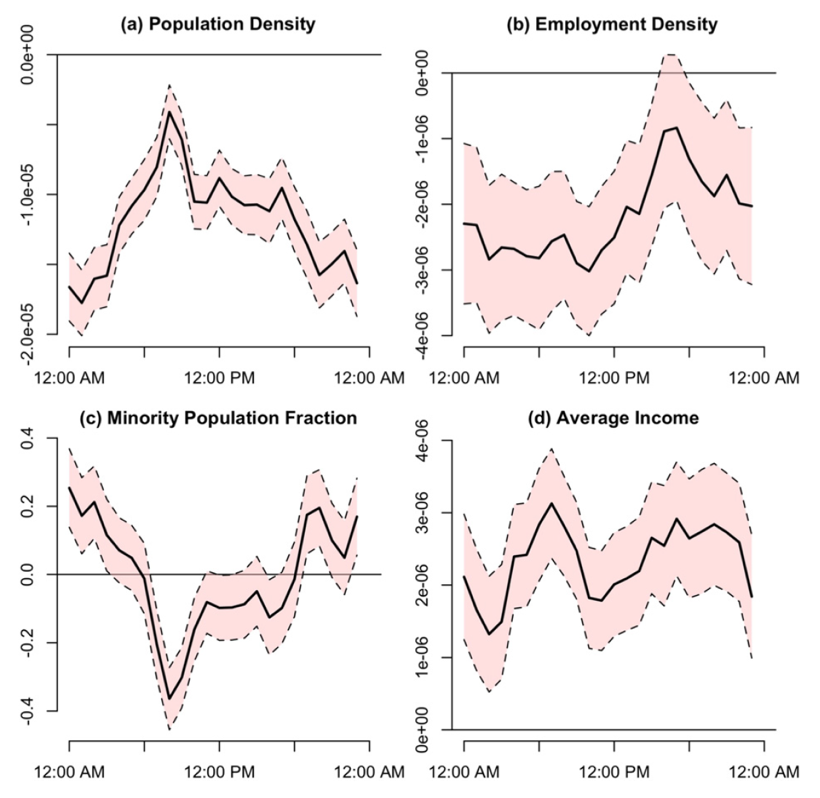
\includegraphics[width=0.6\linewidth]{hughes1.png}
%  \caption{Coefficient estimates and 95\% confidence interval of spatial error model for (a) population density, (b) employment density, (c)minority population fraction, and (d) average income \cite{hughes2016transportation}.}
%  \label{fig:hughes1}
%\end{figure*}
\begin{figure}[!tbp]
  \centering
  \begin{minipage}[b]{0.45\textwidth}
    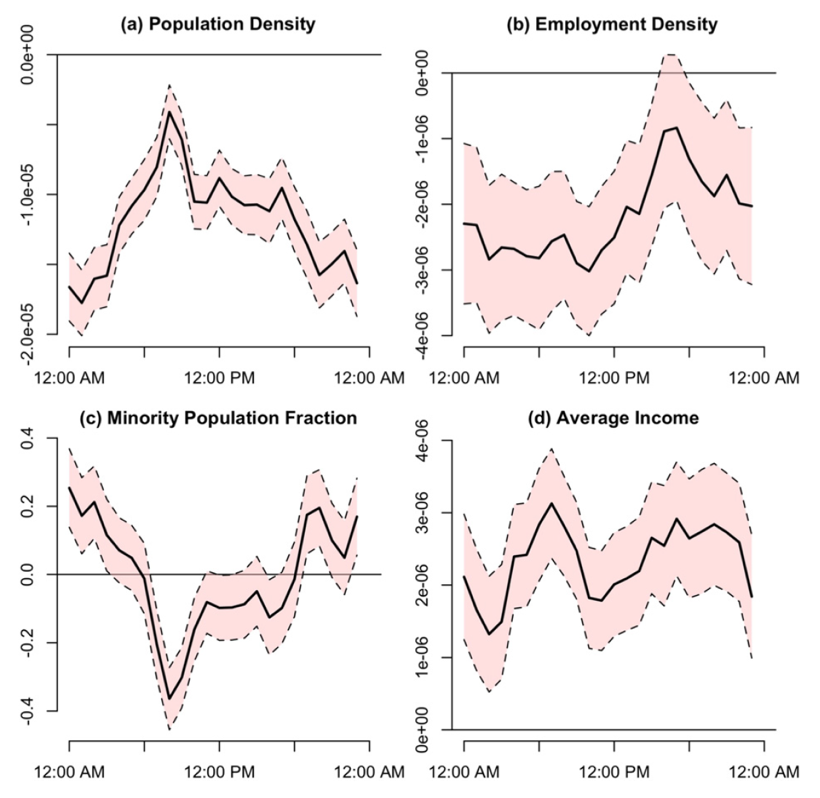
\includegraphics[width=\textwidth]{hughes1.png}
    \caption{Coefficient estimates and 95\% confidence interval of spatial error model for (a) population density, (b) employment density, (c)minority population fraction, and (d) average income \cite{hughes2016transportation}.}
    \label{fig:hughes1}
  \end{minipage}
  \hfill
  \begin{minipage}[b]{0.45\textwidth}
    \centering
    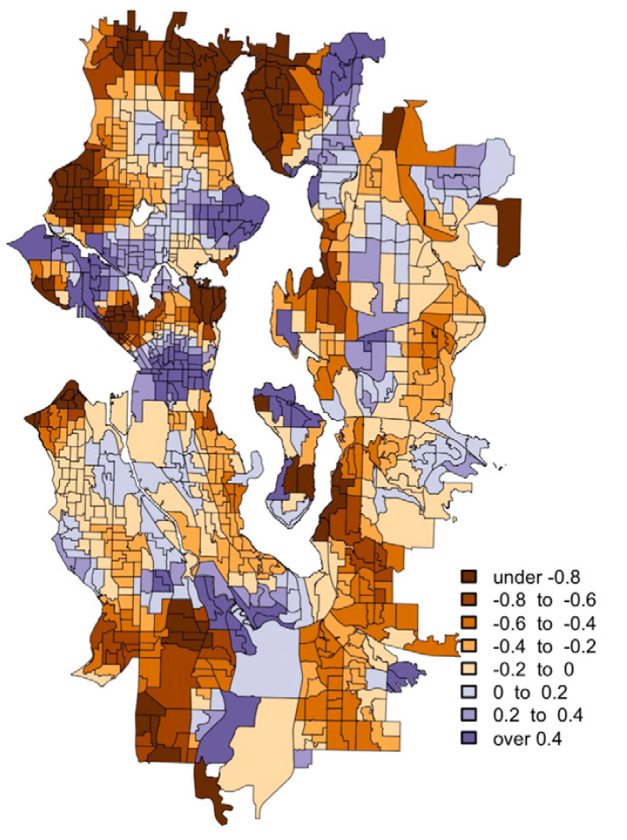
\includegraphics[height=2.9in]{hughes2.png}
    \caption{Coefficients for minority fraction from geographically weighted regression. Purple indicates a positive association between expected waiting time and minority fraction; gold indicates a negative association \cite{hughes2016transportation}.}
    \label{fig:hughes2}
  \end{minipage}
\end{figure}
% across the 24 models representing each hour of the day
Hughes and MacKenzie \cite{hughes2016transportation} investigated the relationships between wait times for UberX and socioeconomic indicators at census block group (CBG) level in Greater Seattle area. They obtained wait times by making UberX requests through Uber API using quasi-randomly selected locations throughout Greater Seattle. They collected about 1 million data points over a two-month period in 2015. Socioeconomic data including population density, employment density, average income, and minority population fraction was collected from the American Community Survey 5-year estimates (ACS). 

They first fitted a regression model with mean waiting times in a CBG as dependent variable and socioeconomic attributes as independent variables. Using a Moran index test, they found significant spatial dependencies among waiting times in different CBG. Subsequently, they developed a spatial error model for each hour of the day to incorporate spatial effect into regression. Results showed that after adjusting the other covariates, higher population density and employment density were associated with shorter waiting time, but that the fraction of minorities in a block group did not significantly associated with waiting times, and that the relationship between these two variables varied between positive and negative throughout the day (Figure \ref{fig:hughes1}). In addition, higher average income is associated with longer wait times, suggesting that low-income areas enjoy better services. 
Geographically weighted regression (GWR) \cite{fotheringham2003geographically} was used to inform different impacts of each socioeconomic variable on different regions. GWR results showed that the relationship between the fraction of minority and wait times is mostly negative. They concluded that ``white and wealthy'' areas do not necessarily enjoy a better TNC service in terms of wait times.

%\begin{figure*}[h]
%  \centering
%  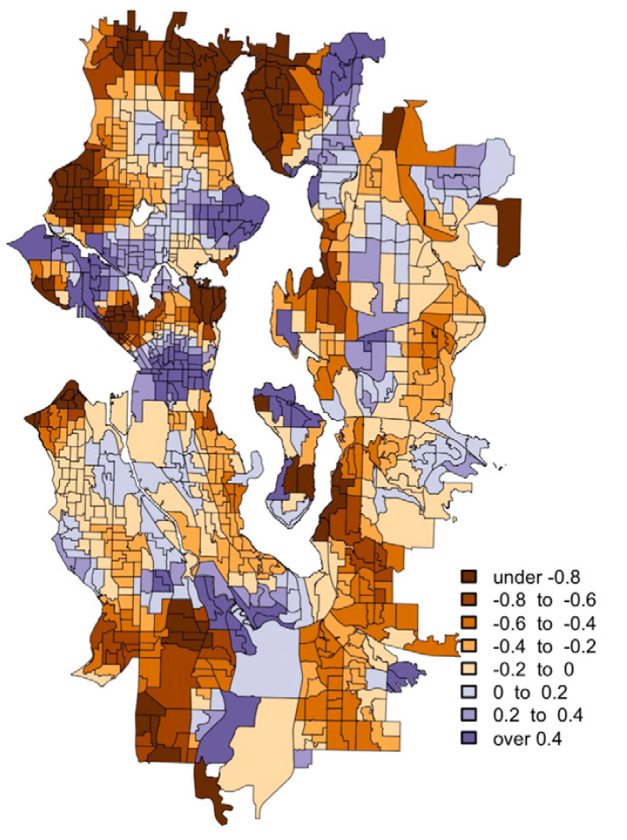
\includegraphics[width=0.35\linewidth]{hughes2.png}
%  \caption{Coefficients for minority fraction from geographically weighted regression. Purple indicates a positive association between expected waiting time and minority fraction; gold indicates a negative association \cite{hughes2016transportation}.}
%  \label{fig:hughes2}
%\end{figure*}

The strength of this study is that it examined both spatial and temporal variations of the effects of different variables (e.g., minority fraction) on TNC waiting times. An interesting addition to this study is to include factors describing the urban form, such as road network into analysis into analysis. For example, the authors found out that higher income is associated with longer waiting time. It is possible that areas with dense road networks tend to experience shorter waiting times, and high-income individuals tend to live in areas with sparse road networks. If this is case, it implies that current urban infrastructure may contribute to the inequalities of new mobility services. For the same reason, it is unclear if the relationships found in this study will generalize to other cities, of which urban forms (e.g., road network, crime rate, employment density, etc.) differ from Seattle. 

Example 1 and Example 2 both examined the equity of service provision in terms of a single indicator (service area coverage and waiting times). These two examples sought to evaluate \textit{equity of opportunity}. While waiting times and docking station locations are important, they do not fully imply the disparities in actual use. For example, individuals without a smartphone cannot use shared bikes even if the docking station is located close to them. The following example approaches this problem from another perspective, namely, focusing on evaluating the \textit{equity of outcome}.  

\paragraph{Example 3: Inequalities in usage of a public bicycle sharing}
Ogilvie and Goodman \cite{ogilvie2012inequalities} explored the correlation between the usage of a bikeshare system in London and socioeconomic attributes. The dataset they use is the anonymized user registration data of a bikeshare system. They examined two dependent variables separately: mean number of trips made by a registered user per month (continuous) and whether a registered user has ever made any trip (binary). They constructed a series of independent variables from the registration data, including gender, place of residence, income deprivation (English Indices of Deprivation) at the level of the Lower Super Output Area (LSOA, a base unit of UK census data), non-White percentage of residential LSOA, distance from residence to nearest bike station, number of stations within 250m of residence, month of registration, etc. 

% percentage of LSOA population commuting by cycling,
The authors employed linear regression to examine the relationship between “mean number of trips per month” and independent variables, and logistic regression to examine the relationship between “ever made any trip” and independent variables. Spatial autocorrelation was accounted for using maximum likelihood estimation. Regression results showed that female users made fewer trips than males per month and users in more deprived areas are less likely to live close to a bike station. After adjusting for the distance from residential area to station, those in more deprived areas made more trips than those in the least deprived areas. They concluded that disparities exist in usage of the system across population, and the system has potentials to fulfill unmet meet if services expand to more deprived areas. 

This study examined the equity of individual-level bikeshare usage. Although the authors found that female users tend to have fewer trips than male users, they cannot determine the cause of this observed relationship. It could be that females tend to have fewer bike trips at night or to regions with high crime rates due to safety concerns. After adjusting for crime rate or time of day, the association between bike usage and gender may change. This brings up another limitation of this research resulted from the use of automatically collected data from bikeshare system. The authors did not have control over the data collection process, so what they could study is also limited. Moreover, constrained by the data availability, the authors had to use area-level socioeconomic variables derived from the postcode of registration debit or credit card. It is thus unclear whether the conclusions would still hold if individual-level variables were available. The temporal scale of the data (7 months) limits the possibility to explore seasonal effects of bike usage. 

% It could be that the authors did not have access to information on when the trips were performed, so the further analysis based on time of day was not possible. 

%This study exposes the tension between privacy and transparency of new mobility data. Equity studies benefit  from individual-level user data, nevertheless, privacy concerns restrict the sharing of such data to the general public. Research is needed to create high quality and privacy-preserving datasets for and beyond transportation equity studies. 


\paragraph{Advantages and limitations of correlational research for equity studies}
By using correlational research, researchers can examine the relationships between transportation provision (or usage) and a wide range of variables collected from various sources. This is especially true when large amount of automatically collected data (e.g., smart card data, bikeshare trip database) is available.  Correlational research is appropriate when researchers are unable to manipulate the variables due to practical or ethical reasons. For example, in equity studies, area-level variables such as average income of a CBG is not controllable. 

One limitation of correlational research is that a significant correlation does not allow the researcher to determine a causal relationship, because there could be many factors that the researcher did not study but contribute to the correlation. And these factors could be independent of mobility service provision. Further inquiry is needed to corroborate the findings from a correlational study. Another limitation is that correlational research heavily depends on data availability and data quality, as discussed in Example 3. 
\subsection{Experimental Research}
Experimental research enables researchers to identify causal relationship. In an experiment design, the researcher seeks to fully control the environment conditions so that variables of interest can be manipulated, while other variables are controlled (or randomized) across conditions. In this way, the effects of variables of interest can be tested by comparing between two or more conditions. Unlike correlational research, experimental research strictly controls for the impacts of variables not of interest, thus allowing the effects of variables of interest to be measured upon the outcome \cite{lazar2017research}. 

\paragraph{Example: Racial and gender discrimination in transportation network companies}
Ge et al.\cite{ge2016racial} studied the racial and gender discrimination in Transportation Network Companies (TNCs). They undertook two randomized control trails, hailing about 1500 rides in Seattle and Boston and recording service quality indicators. In the  Seattle experiment, the treatment is race. Eight RAs (two African American females, two white females, two African American males, and two white males) were hired to request rides. Measures including estimated waiting times, acceptance time (time between trip request and acceptance), actual waiting times (time between acceptance and arrival), trip cancellation rate, trip duration, costs, and ratings were recorded by screenshots for each trip. To control for variables not of interest, the authors adopted a number of strategies. The RAs are undergraduate students, avoiding confounding factors such as age. They were given the identical smartphones using the same carriers, and received the same data collection instructions. The RAs were instructed to minimize their interactions with the driver, preventing the introduction of factors that influence ratings and travel time. Specific routes were developed to control for pick-up locations and travel duration. These routes were randomly assigned to RAs. RAs were also instructed to travel after evening rush hours from Mondays to Thursdays. Ordinary least squares regression (OLS) results showed that acceptance time is longer for African American riders than white riders for both UberX and Lyft. 

In the Boston experiment, the authors adopted a within-group design. They hired eight RAs with a range of ethnic backgrounds summoning UberX or Lyft rides in Boston, each requesting rides under a “white-sounding” name and a “distinctively black name”. This change in design aims to control the differences in data collection practices among RAs. In this case, the treatment is whether the rider has a black sounding name. Other aspects of experiment design are similar to those of the Seattle experiment. OLS results showed that riders with African American-sounding names experienced more frequent trip cancellations, and that African American males have higher cancellation rates than white males. Further analysis revealed that trip cancellations concentrated in pickup locations with low population density. They concluded that racial discrimination exists in TNC services in Seattle and Boston.


\paragraph{Advantages and limitations of experimental research for equity studies}
Experimental research allows for drawing causal conclusions. This is because experiments are conducted in controlled conditions and researchers can claim that the changes in outcomes are caused by the variable of interest. 

Experimental research has notable limitations. First, the requirement that controlling all variables that might influence the outcomes is sometimes not realistic. This is especially true for experiments conducted in a natural environment. For example, in Ge et al.’s Seattle experiment \cite{ge2016racial}, there are variances in the data collection practices (e.g., the time lag between taking screenshots and sending requests) among RAs. This influences the measurement of outcome variables. Second, compared to automatically collected data or survey data, experiments are often not able to produce large amount of data. Data collection in experiments is often expensive and labor-intensive. Finally, although experimental research can determine causal effects (e.g., racial discrimination exists in TNC services in Seattle), it cannot unveil the reasons why the outcome occurred (e.g., why TNC drivers discriminate against certain races). Further investigation through other research methods (e.g., interviews) is needed to understand the phenomenon.  
\begin{figure}[!tbp]
  \centering
  \begin{minipage}[b]{0.48\textwidth}
    \centering
    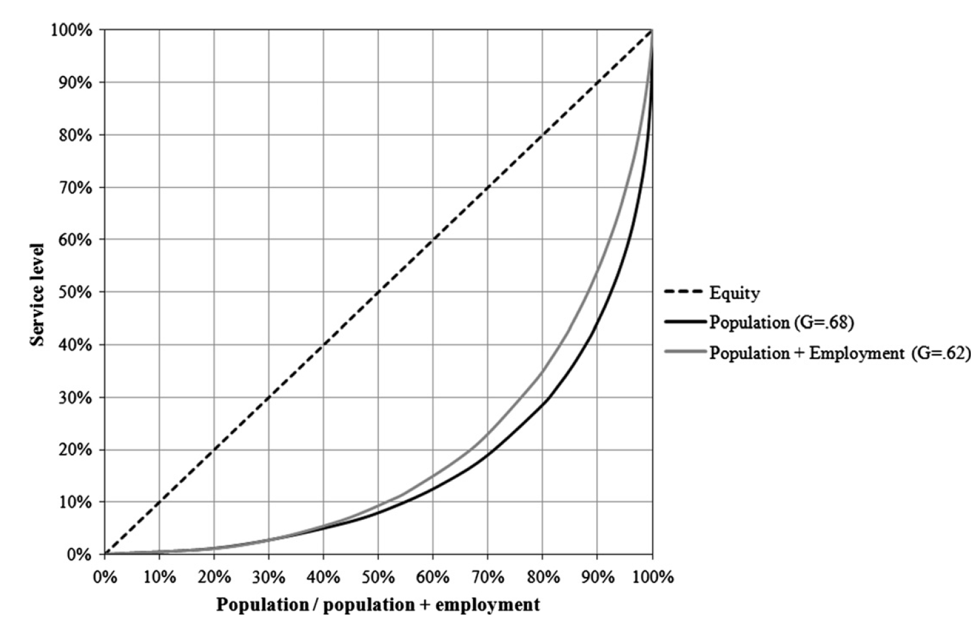
\includegraphics[width=\textwidth]{gini2.png}
    \caption{Use Lorenz curves to compare the equity of public transport service level to demand (population and employment) \cite{delbosc2011using}.}
    \label{fig:gini2}
  \end{minipage}
  \hspace{2cm}
  \begin{minipage}[b]{0.34\textwidth}
    \centering
    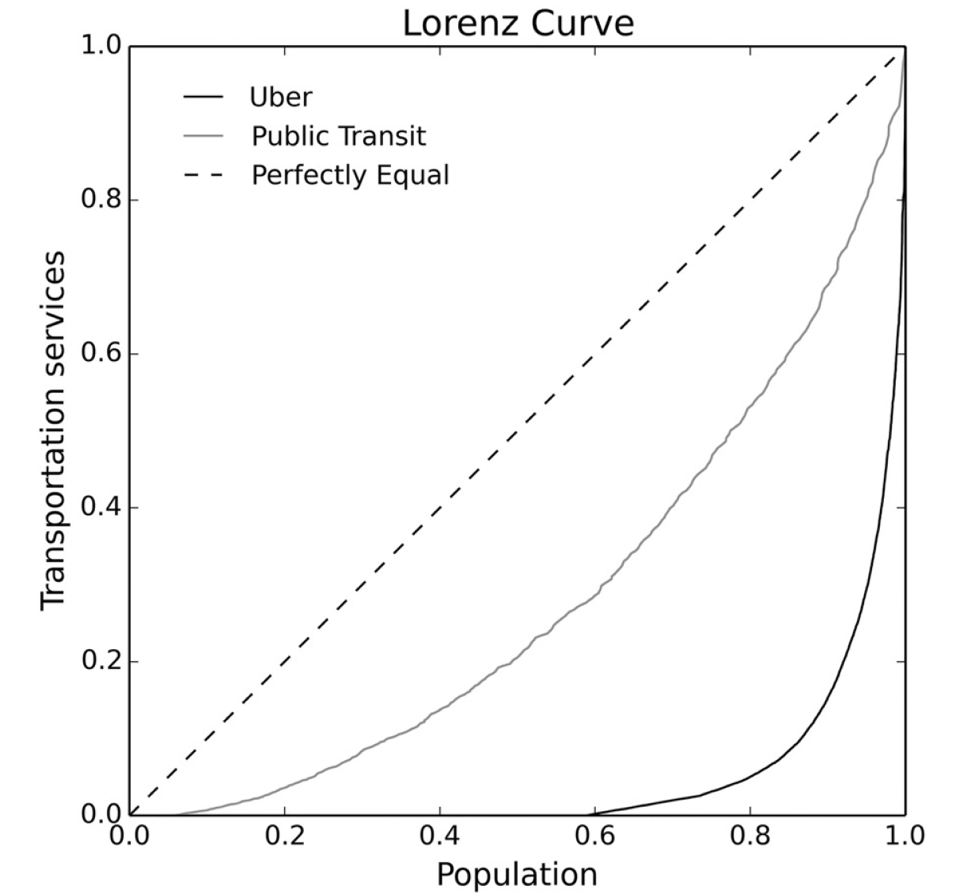
\includegraphics[width=\textwidth]{gini3.png}
    \caption{Use Lorenz curves to compare the equity of public transport and Uber  service level to population \cite{jin2019uber}.}
    \label{fig:gini3}
  \end{minipage}
\end{figure}
\subsection{Equity Metrics}
Metrics that measure the distribution of some mobility system impacts (e.g., service level) have been widely adopted in transportation equity evaluation. Unlike statistical tests which focus on the discovery of discrimination or inequalities, metrics directly gauge the degree of equity by a single value. Equity metrics used in transportation equity research differ but overlap with those used in fairness in machine learning research. The similarities between them partially arise from the fact that both fields borrowed ideas from other domains such as social welfare and economics. For example, Gini coefficient (or Gini index), initially proposed to represent cumulative income and wealth distribution across a population, is one of the most popular equity metrics used in transportation to gauge the equity of transportation resource allocation \cite{ricciardi2015exploring}.  However, Gini index has not yet received much attention in machine learning community \cite{speicher2018unified}. Perhaps this is because fairness in machine learning research has primarily concentrated on classification problems that used in credit scoring, profiling of potential suspects, hiring, etc., for which other metrics are more appropriate. On the other hand, there are a few metrics, such as the “80\% Rule” \cite{useeoc}, were used in both communities \cite{feldman2015certifying}. The following examples introduce the use of Gini index and the "80\% Rule” in transportation equity. 

\paragraph{Example 1: Using Lorenz curves to assess public transport equity in Melbourne}
Delbosc and Currie \cite{delbosc2011using} proposed to use Gini index as an equity metric of public transit service provision. A Lorenz curve is a graphical representation of Gini index. The figure below (see Figure \ref{fig:gini2}) illustrates an example of a Lorenz curve representing the cumulative income across a population. The perfect equitable income distribution is plotted as the dashed line (line of equity) and an inequitable distribution of income is represented by the solid curve (Lorenz curve). A point on the solid curve can be interpreted as X percent (e.g., 70\%) of population shares about Y percent (e.g., 25\%) of the total income of the population. Gini index is the ratio of the area between the line of equity and the Lorenz curve (A), divided by the total area under the line of equity (A+B). 
%A Gini index of zero signifies perfect equity, whereas Gini index of one expresses the maximum inequality. 



%\begin{figure*}[h]
%  \centering
%  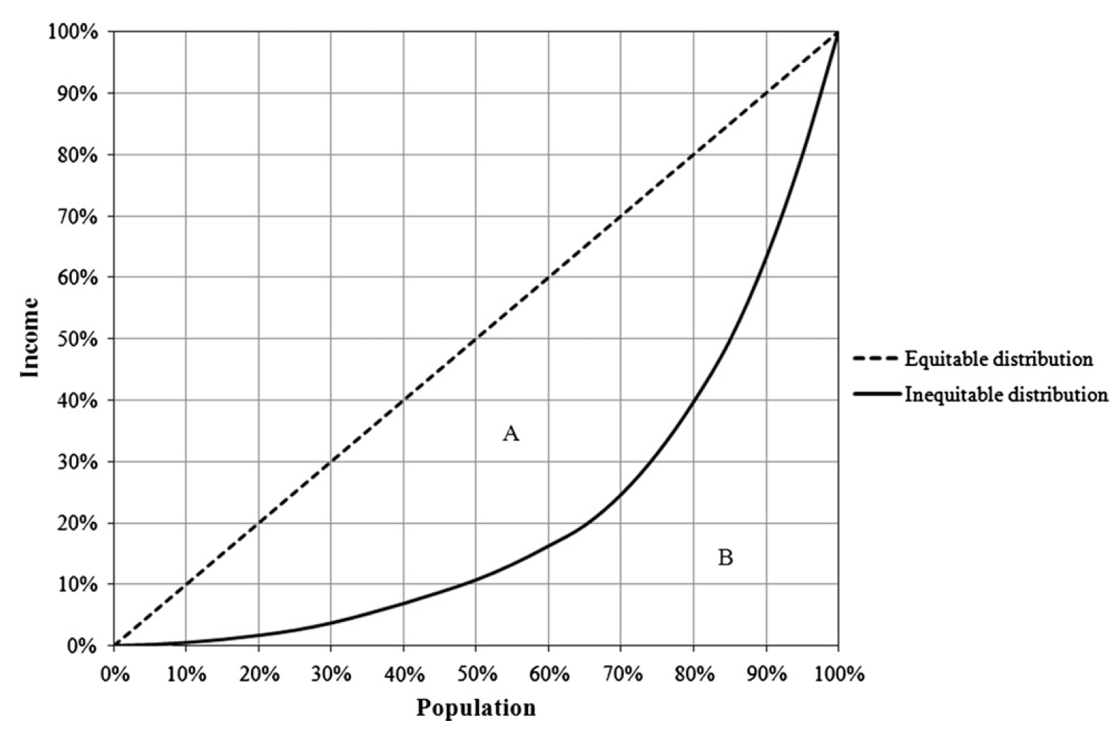
\includegraphics[width=0.6\linewidth]{gini1.png}
%  \caption{Gini coefficient is equal to the area between line of equity and the Lorenz curve (A), divided by the total area under the line of equity (A+B) \cite{delbosc2011using}.}
%  \label{fig:gini1}
%\end{figure*}

Delbosc and Currie applied a gini index to compare the equity of public transport service level to a proxy of demand (population and employment) in Melbourne. Service level of a census tract is expressed as a composite index taking into account bus, tram, and rail service areas and frequency. Using the service level index and the population of each census tract, the authors generated the first Lorenz curve (black solid curve) as shown in Figure \ref{fig:gini2}. The Gini index is 0.68 for overall population in Melbourne. This can be interpreted as 70\% of the population shares 19\% of the public transport services. A second Lorenz curve (a grey solid curve) was calculated, taking into account the employment density. The Gini index for total population and employment is 0.62, appearing more equitable than the first curve. Nevertheless, these two curves suggest that inequalities exist in public transit, with only a small portion of the population enjoying the majority of transit services. 

%\begin{figure*}[h]
  %\centering
  %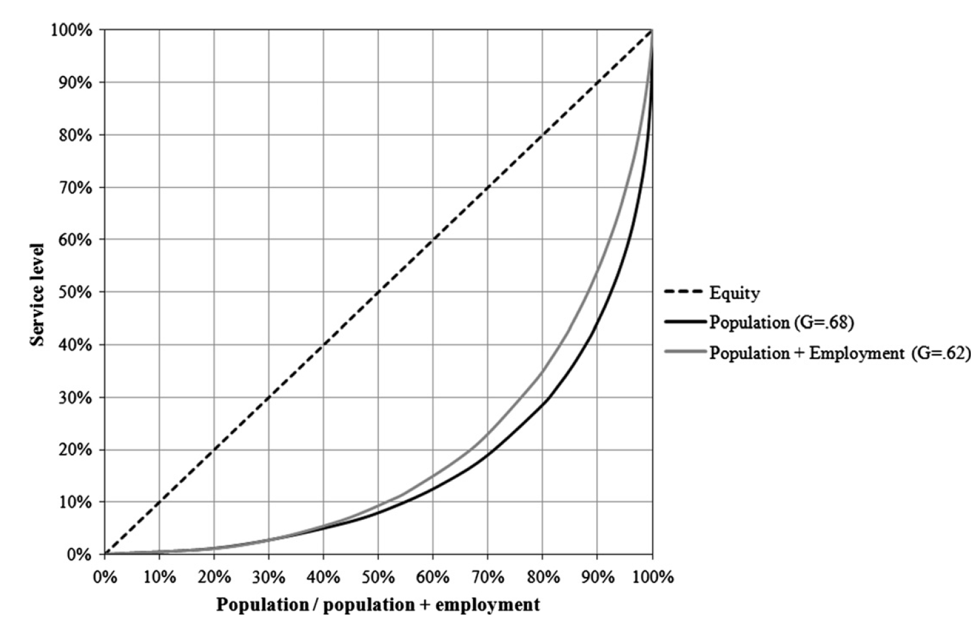
\includegraphics[width=0.6\linewidth]{gini2.png}
  %\caption{Use Lorenz curves to compare the equity of public transport service level to demand (population and employment) \cite{delbosc2011using}.}
%  \label{fig:gini2}
%\end{figure*}



In this example, the Gini index serves as a measure of horizontal equity, that is,  providing equal resources to those equal in need. The need for transportation supply of each census tract is approximated by population and employment density. So the perfect equitable distribution is that every unit of population and jobs shares the same transport resources. The need of special demographic groups (vertical equity) is not considered. 

\paragraph{Example 2: Using Lorenz curves to access the equity of Uber and public transit in New York City}
%\begin{figure*}[h]
%  \centering
%  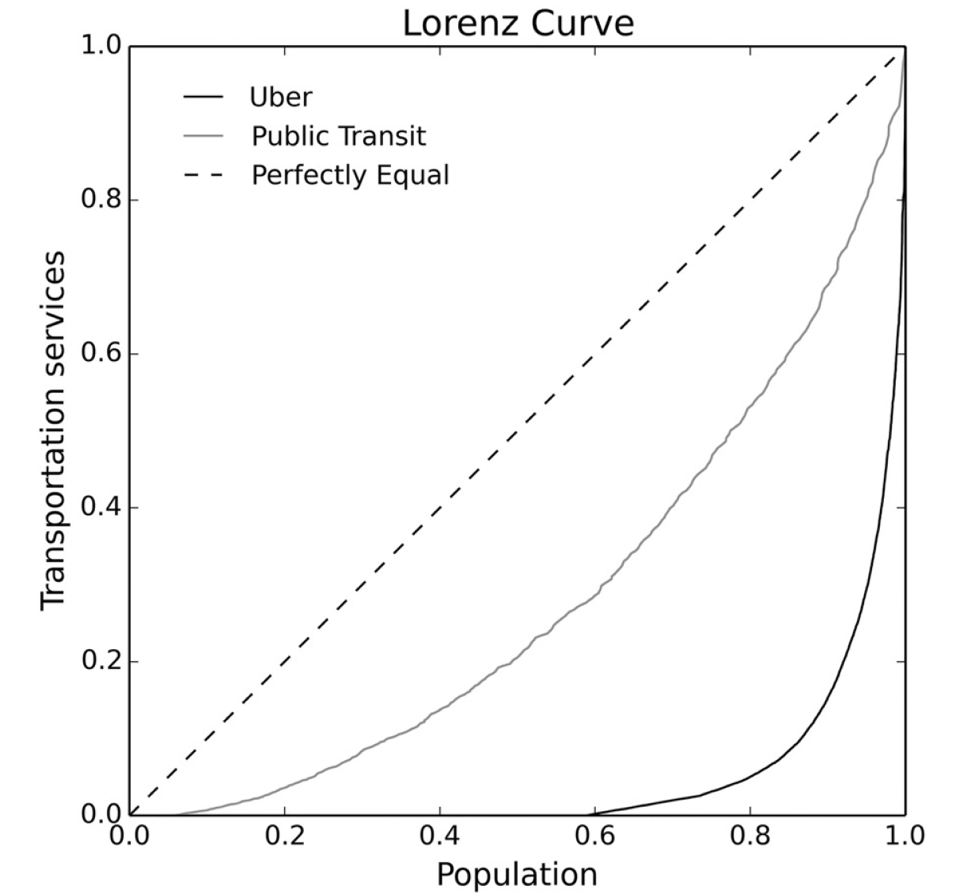
\includegraphics[width=0.4\linewidth]{gini3.png}
%  \caption{Use Lorenz curves to compare the equity of public transport and Uber  service level to population \cite{jin2019uber}.}
%  \label{fig:gini3}
%\end{figure*}
Most recently, Jin et al. \cite{jin2019uber} employed Lorenz curves and Gini index to study the equity of Uber services in New York City (see Figure \ref{fig:gini3}).  They calculated service level for Uber and public transit using a similar approach as Delbosc and Currie \cite{delbosc2011using}. Their results suggested that Uber is less equitable than public transit: 20\% of population shares the 95\% of Uber services. 

They further compared Gini indexes of different boroughs for public transit and public transit + Uber (see Table \ref{fig:gini4}). The results (see Table \ref{fig:gini4}) shows that with Uber, the Gini index of the whole city reduced by about 0.03 on weekdays and by about 0.008 on weekends. This implies that Uber has insignificant impact on the transportation equity of New York City. 


\begin{figure*}[tb]
  \centering
  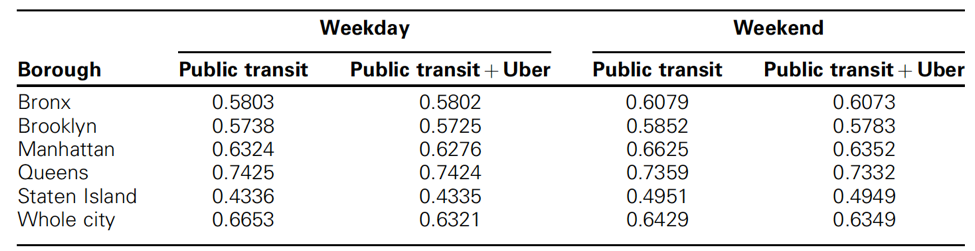
\includegraphics[width=0.8\linewidth]{gini4.png}
  \captionof{table}{Gini coefficient without and with Uber \cite{jin2019uber} }
%   \caption{Gini coefficient without and with Uber \cite{jin2019uber}.}
  \label{fig:gini4}
\end{figure*}

This study exemplifies how Gini index can be used to compare transportation equity across regions and across modes. This is possible because Gini index has several desirable features:  it does not depend on the size of the population, the overall transit supply level, or the geographic units. For example, Gini index can be used to examine the equity of a neighborhood, a city, or a country. And it enables the comparison of equity between a city with high level of transit supply and one with low supply. 

One limitation of Gini index is its heavy reliance on data. As Jin et al. noted, the main reason to choose New York City as study area is data availability. Beyond availability, all data sources have limitations (e.g., census data is not up-to-date) that would be calculated into Gini index. Another limitation lies in the way the service level is calculated. Studies that employed Gini indexes tend to use different methods to calculate service level \cite{feng2014trade}. It is unclear whether changing the service level indicator will significantly affect Gini index. These two limitations suggest that Gini indexes should be interpreted with caution. 

\paragraph{Example 3: Evaluation of the equity of bikeshare system accessibility}
Meng \cite{meng2018evaluation} applied the “80\% Rule” to evaluate access equity of a bikeshare system in Chicago. The “80\% Rule” was advocated by the US Equal Employment Opportunity Commission to detect disparate impacts in employee selection procedures. The 80\% Rule states that if the selection rate for minorities is less than 80\% of the rate of non-minorities, the procedure is deemed to be discriminatory \cite{useeoc}. Similar to Ursaki and Aultman-Hall (see Example 1 of Section \ref{sec:correlation}), the analysis is based on the locations of docking stations. The author created a 0.25-mile buffer around each station as service area, and calculated the demographic characteristics (i.e., race, gender, education, language proficiency, and income level) of population inside each service area. For each station, the equity metric based on the 80\% Rule is calculated as follows:


\begin{equation}
    Ratio = \frac{Number \  of \  minorities / Total \ number \ of \ minorities}{Number \ of \ non-minorities / Total \ number \ of \ non-minorities}
\end{equation}

The results show that more than 33\% of the stations have ratios below 0.8 for all demographic characteristics (except for gender) under examination.

There are several limitations of this study. First, instead of providing a city-level ratio, the authors computed station-level ratios and examined equity using the percentage of stations that violate the 80\% Rule. This approach is problematic when the stations are not equally distributed. It is possible that a majority of the stations are all located in a small portion of the city and they tend to have similar ratios. Second, docking station placement cannot sufficiently represent access to bikeshare, as discussed in Example 1 of Section \ref{sec:correlation}. Despite these weaknesses, this study serves as a typical example of using fairness metrics to evaluate vertical equity in new mobility systems. 

\paragraph{Advantages and limitations of equity metrics}
Equity metric provides a single measure of equity, making it possible to track trends over time and conduct comparative studies between cities. It is easier for non-experts to interpret compared to statistical tests, therefore suited for conveying evaluation results to broader audience.

However, the reliability of metrics heavily depends on the quality of data sources. Moreover, different metrics often reflect competing goals. For example, Gini index measures horizontal equity, emphasizing individuals with equal ability or need gets equal resources. The 80\% Rule shares a similar spirit of group fairness \cite{feldman2015certifying}, which advocates for equal resource distribution across difference demographic groups.  The choice of metrics may significantly affect evaluation results, so the use of multiple metrics is important.   

\subsection{Other methods}
Apart from the three research methods described above, surveys, interviews, and focus groups have been used for transportation equity studies. These methods can be used to develop a deeper understanding of why inequalities exist based on the opinions, attitudes, and experiences from stakeholders of mobility systems. For example, McNeil, Nathan, et al. \cite{mcneil2017breaking} conducted a survey of residents living in underserved neighborhoods with bikesahre stations. The findings revealed that minority respondents have more barriers, for example, costs of membership, to using shared bikes than non-minorities. This helps to explain why providing adequate spatial access to disadvantaged neighborhoods alone is not enough to address the disparities in actual use. 

\section{Transportation Equity and Fairness in Machine learning}

In examining the fairness (equity) definitions from transportation equity community and fair machine learning (FairML) community, we observe that a natural mapping between them can be established, though further effort is needed to create a consistent mapping between concepts in one domain to the other. \textit{Horizontal equity} echoes the spirit of \textit{individual fairness} (similar people should be treated similarly). \textit{Vertical equity} resembles \textit{group fairness} (sensitive attributes should be independent from outcomes). This is true in cities where there is an uneven distribution of transport supply across different socioeconomic groups. Vertical equity encourages compensating for such inequalities by policies favoring disadvantaged groups. This aligns with group fairness that the level of transportation supply in a city should be the same across different groups. Vertical equity and group fairness are only ``roughly'' related because by definition, group fairness stresses ``independence'' between sensitive attributes and outcome, whereas vertical equity does not.   

%\begin{figure*}[h]
%  \centering
%  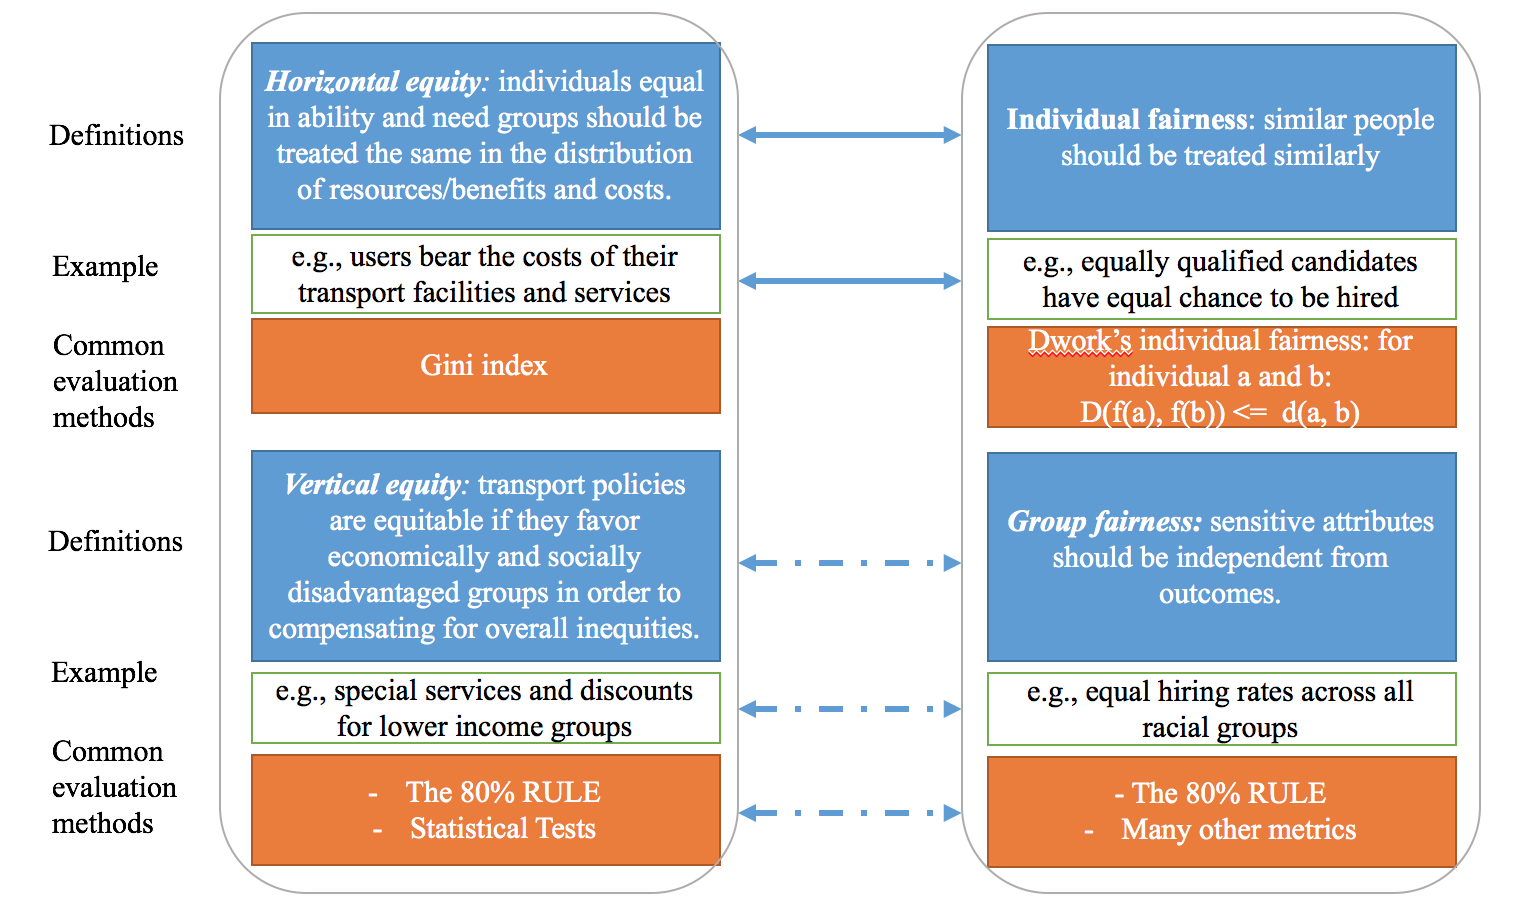
\includegraphics[width=0.8\linewidth]{mapping.png}
%  \caption{Mapping of concepts, examples, and methods between transportation equity (left) and fair machine learning (right)}
%  \label{fig:mapping}
%\end{figure*}

The most commonly used method for evaluating horizontal equity is Gini index. It has not attracted much attention in machine learning community. This may be partially due to the fact that not much attention has been paid to resource allocation problems in fair machine learning research. On the other hand, machine learning community has developed a few metrics for individual fairness. Individual fairness requires that the ``similarity'' between a pair of individuals from two demographic groups respectively has to be defined. For example, in making hiring decisions, the algorithm has to possess perfect knowledge of how to compare the ``qualification'' of two individuals. This is often not realistic in  practice and we have to come up with a suitable similarity metric that is best agreed upon among domain experts of a task. Theoretically, individual fairness can be used to evaluate horizontal equity. For example, in a simplified shared bike allocation problem, we use population and employment density as the demand for bikes. Then the differences in demand between two areas $a$ and $b$ can be expressed as $d(a, b)$ according to some similarity function $d$. Suppose we have an algorithm assigning bikes to areas, the number of bikes that area $a$ and $b$ will get is $f(a)$ and $f(b)$, respectively. A fair allocation satisfying individual fairness requires that for every two pairs of areas in the city: $D(f(a) , f(b)) <= d(a,b)$, where $D$ is another similarity function. The difficulty again, lies in the fact that we do not have perfect knowledge to determine the similarity in demand between two areas. 

The majority of transportation equity research focuses on vertical equity. Likewise, more attention has been devoted to group fairness than individual fairness in machine learning community. Transportation equity heavily employs statistical tests for equity analysis, which is appropriate for discovering unfairness. Machine learning uses fairness metrics much more often, because metrics allow researchers to reduce achieving fairness goals to a much simpler problem: minimizing a value that represents unfairness. This is also valid in terms of algorithm design. In fact, some metrics, such as the 80\% Rule, have been used in both communities. This connection may open great possibilities for bridging these two domains.   

Fair machine learning community focuses almost exclusively on methods, whereas transportation equity concerns more about applications, policies, and interventions. Although fair machine learning approaches hold great promises in optimizing resource allocation in mobility settings, there is a long way to go to design, deploy, and evaluate a fairness-aware data-driven system as a real-world application. At the end of this paper, I hope to highlight the urgency of convergence of these two fields. Ultimately, researchers with knowledge in both fields, practitioners, policy-makers, and citizens should work together towards a common goal: a fair and effective transportation system for  all citizens. 


\section{Conclusion}
% \looseness-1
This paper summarized the findings and methods of equity studies in mobility systems, with a focus on new mobility systems. For new mobility services, it is generally agreed that disparities exist in the access and use of docked bikeshare system, but the equity implications of ride-hailing are still unclear. Further research is needed to understand how to deliver a more equitable new mobility system to serve the need of different groups. Many research methods have been employed in transportation equity studies. Different methods vary in their objectives, strengths and weaknesses. Correlational research can exploit a wide range of data sources and discover associations among many factors, but it cannot determine causal relationships. Equity metrics enable comparative studies among cities and assessment of changes over time, but their reliability is highly dependent on data. Experimental research can produce reliable findings, but is expensive and difficult to control all extraneous variables. The choice of research methods depends on research goals, and multiple methods can be used together to complement each other. 

Given the similarities in objectives, concepts, and methods between transportation equity community and fairness in machine learning community, bridging these two domains together holds promise to enable multi-disciplinary breakthroughs. 


\begin{thebibliography}{10}
\itemsep=1pt
\begin{small}

\bibitem{AbiteboulHVBook}
Serge Abiteboul, Richard Hull, and Victor Vianu.
\newblock {\em Foundations of Databases}.
\newblock Addison-Wesley, 1995.

\bibitem{ainy2015approximated}
Eleanor Ainy, Pierre Bourhis, Susan~B Davidson, Daniel Deutch, and Tova Milo.
\newblock Approximated summarization of data provenance.
\newblock In {\em Proceedings of the 24th ACM International on Conference on
  Information and Knowledge Management}, pages 483--492. ACM, 2015.

\bibitem{antenucci2018constraint}
Dolan Antenucci and Michael Cafarella.
\newblock Constraint-based explanation and repair of filter-based
  transformations.
\newblock {\em Proceedings of the VLDB Endowment}, 11(9):947--960, 2018.

\bibitem{avin2005identifiability}
Chen Avin, Ilya Shpitser, and Judea Pearl.
\newblock Identifiability of path-specific effects.
\newblock In {\em Proceedings of International Joint Conference on Artificial
  Intelligence}, pages 357--363, 2005.

\bibitem{bertossi2017causes}
Leopoldo Bertossi and Babak Salimi.
\newblock Causes for query answers from databases: Datalog abduction,
  view-updates, and integrity constraints.
\newblock {\em International Journal of Approximate Reasoning}, 90:226--252,
  2017.

\bibitem{DBLP:series/synthesis/2011Bertossi}
Leopoldo~E. Bertossi.
\newblock {\em Database Repairing and Consistent Query Answering}.
\newblock Synthesis Lectures on Data Management. Morgan {\&} Claypool
  Publishers, 2011.

\bibitem{calders2009building}
Toon Calders, Faisal Kamiran, and Mykola Pechenizkiy.
\newblock Building classifiers with independency constraints.
\newblock In {\em Data mining workshops, 2009. ICDMW'09. IEEE international
  conference on}, pages 13--18. IEEE, 2009.

\bibitem{chapman2009not}
Adriane Chapman and HV~Jagadish.
\newblock Why not?
\newblock In {\em Proceedings of the 2009 ACM SIGMOD International Conference
  on Management of data}, pages 523--534. ACM, 2009.

\bibitem{chouldechova2017fair}
Alexandra Chouldechova.
\newblock Fair prediction with disparate impact: A study of bias in recidivism
  prediction instruments.
\newblock {\em Big data}, 5(2):153--163, 2017.

\bibitem{corbett2017algorithmic}
Sam Corbett-Davies, Emma Pierson, Avi Feller, Sharad Goel, and Aziz Huq.
\newblock Algorithmic decision making and the cost of fairness.
\newblock In {\em Proceedings of the 23rd ACM SIGKDD International Conference
  on Knowledge Discovery and Data Mining}, pages 797--806. ACM, 2017.

\bibitem{courtland2018bias}
Rachel Courtland.
\newblock Bias detectives: the researchers striving to make algorithms fair.
\newblock {\em Nature}, 558, 2018.

\bibitem{dwork2012fairness}
Cynthia Dwork, Moritz Hardt, Toniann Pitassi, Omer Reingold, and Richard Zemel.
\newblock Fairness through awareness.
\newblock In {\em Proceedings of the 3rd innovations in theoretical computer
  science conference}, pages 214--226. ACM, 2012.

\bibitem{galhotra2017fairness}
Sainyam Galhotra, Yuriy Brun, and Alexandra Meliou.
\newblock Fairness testing: testing software for discrimination.
\newblock In {\em Proceedings of the 2017 11th Joint Meeting on Foundations of
  Software Engineering}, pages 498--510. ACM, 2017.

\bibitem{glavic2007data}
Boris Glavic and Klaus Dittrich.
\newblock Data provenance: A categorization of existing approaches.
\newblock {\em Datenbanksysteme in Business, Technologie und Web (BTW
  2007)--12. Fachtagung des GI-Fachbereichs" Datenbanken und
  Informationssysteme"(DBIS)}, 2007.

\bibitem{hardt2016equality}
Moritz Hardt, Eric Price, Nati Srebro, et~al.
\newblock Equality of opportunity in supervised learning.
\newblock In {\em Advances in neural information processing systems}, pages
  3315--3323, 2016.

\bibitem{kilbertus2017avoiding}
Niki Kilbertus, Mateo~Rojas Carulla, Giambattista Parascandolo, Moritz Hardt,
  Dominik Janzing, and Bernhard Sch{\"o}lkopf.
\newblock Avoiding discrimination through causal reasoning.
\newblock In {\em Advances in Neural Information Processing Systems}, pages
  656--666, 2017.

\bibitem{kusner2017counterfactual}
Matt~J Kusner, Joshua Loftus, Chris Russell, and Ricardo Silva.
\newblock Counterfactual fairness.
\newblock In {\em Advances in Neural Information Processing Systems}, pages
  4069--4079, 2017.

\bibitem{larson2016we}
Jeff Larson, Surya Mattu, Lauren Kirchner, and Julia Angwin.
\newblock How we analyzed the compas recidivism algorithm.
\newblock {\em ProPublica (5 2016)}, 9, 2016.

\bibitem{DBLP:conf/pods/LevyMSS95}
Alon~Y. Levy, Alberto~O. Mendelzon, Yehoshua Sagiv, and Divesh Srivastava.
\newblock Answering queries using views.
\newblock In {\em Proceedings of the Fourteenth {ACM} {SIGACT-SIGMOD-SIGART}
  Symposium on Principles of Database Systems, May 22-25, 1995, San Jose,
  California, {USA}}, pages 95--104, 1995.

\bibitem{adult}
M.~Lichman.
\newblock Uci machine learning repository, 2013.

\bibitem{DBLP:conf/pods/LivshitsKR18}
Ester Livshits, Benny Kimelfeld, and Sudeepa Roy.
\newblock Computing optimal repairs for functional dependencies.
\newblock In {\em Proceedings of the 37th {ACM} {SIGMOD-SIGACT-SIGAI} Symposium
  on Principles of Database Systems, Houston, TX, USA, June 10-15, 2018}, pages
  225--237, 2018.

\bibitem{loftus2018causal}
Joshua~R Loftus, Chris Russell, Matt~J Kusner, and Ricardo Silva.
\newblock Causal reasoning for algorithmic fairness.
\newblock {\em CoRR}, abs/1805.05859, 2018.

\bibitem{meliou2010complexity}
Alexandra Meliou, Wolfgang Gatterbauer, Katherine~F Moore, and Dan Suciu.
\newblock The complexity of causality and responsibility for query answers and
  non-answers.
\newblock {\em Proceedings of the VLDB Endowment}, 4(1):34--45, 2010.

\bibitem{mintz2009distant}
Mike Mintz, Steven Bills, Rion Snow, and Dan Jurafsky.
\newblock Distant supervision for relation extraction without labeled data.
\newblock In {\em Proceedings of the Joint Conference of the 47th Annual
  Meeting of the ACL and the 4th International Joint Conference on Natural
  Language Processing of the AFNLP: Volume 2-Volume 2}, pages 1003--1011.
  Association for Computational Linguistics, 2009.

\bibitem{nabi2018fair}
Razieh Nabi and Ilya Shpitser.
\newblock Fair inference on outcomes.
\newblock In {\em Proceedings of the... AAAI Conference on Artificial
  Intelligence. AAAI Conference on Artificial Intelligence}, volume 2018, page
  1931. NIH Public Access, 2018.

\bibitem{pearl2003causality}
Judea Pearl.
\newblock Causality: models, reasoning, and inference.
\newblock {\em Econometric Theory}, 19(675-685):46, 2003.

\bibitem{pearl2009causality}
Judea Pearl.
\newblock {\em Causality}.
\newblock Cambridge university press, 2009.

\bibitem{pearl2009causal}
Judea Pearl et~al.
\newblock Causal inference in statistics: An overview.
\newblock {\em Statistics Surveys}, 3:96--146, 2009.

\bibitem{DBLP:conf/sigmod/PopaDST00}
Lucian Popa, Alin Deutsch, Arnaud Sahuguet, and Val Tannen.
\newblock A chase too far?
\newblock In {\em Proceedings of the 2000 {ACM} {SIGMOD} International
  Conference on Management of Data, May 16-18, 2000, Dallas, Texas, {USA.}},
  pages 273--284, 2000.

\bibitem{ratner2017snorkel}
Alexander Ratner, Stephen~H Bach, Henry Ehrenberg, Jason Fries, Sen Wu, and
  Christopher R{\'e}.
\newblock Snorkel: Rapid training data creation with weak supervision.
\newblock {\em Proceedings of the VLDB Endowment}, 11(3):269--282, 2017.

\bibitem{ratner2016data}
Alexander~J Ratner, Christopher~M De~Sa, Sen Wu, Daniel Selsam, and Christopher
  R{\'e}.
\newblock Data programming: Creating large training sets, quickly.
\newblock In {\em Advances in neural information processing systems}, pages
  3567--3575, 2016.

\bibitem{raykar2010learning}
Vikas~C Raykar, Shipeng Yu, Linda~H Zhao, Gerardo~Hermosillo Valadez, Charles
  Florin, Luca Bogoni, and Linda Moy.
\newblock Learning from crowds.
\newblock {\em Journal of Machine Learning Research}, 11(Apr):1297--1322, 2010.

\bibitem{roy2014formal}
Sudeepa Roy and Dan Suciu.
\newblock A formal approach to finding explanations for database queries.
\newblock In {\em Proceedings of the 2014 ACM SIGMOD international conference
  on Management of data}, pages 1579--1590. ACM, 2014.

\bibitem{rubin1970thesis}
Donald~B Rubin.
\newblock {\em The Use of Matched Sampling and Regression Adjustment in
  Observational Studies}.
\newblock Ph.D. Thesis, Department of Statistics, Harvard University,
  Cambridge, MA, 1970.

\bibitem{rubin1986statistics}
Donald~B Rubin.
\newblock Statistics and causal inference: Comment: Which ifs have causal
  answers.
\newblock {\em Journal of the American Statistical Association},
  81(396):961--962, 1986.

\bibitem{rubin2008comment}
Donald~B Rubin.
\newblock Comment: The design and analysis of gold standard randomized
  experiments.
\newblock {\em Journal of the American Statistical Association},
  103(484):1350--1353, 2008.

\bibitem{russell2017worlds}
Chris Russell, Matt~J Kusner, Joshua Loftus, and Ricardo Silva.
\newblock When worlds collide: integrating different counterfactual assumptions
  in fairness.
\newblock In {\em Advances in Neural Information Processing Systems}, pages
  6414--6423, 2017.

\bibitem{DBLP:conf/icdt/SalimiB15}
Babak Salimi and Leopoldo~E. Bertossi.
\newblock From causes for database queries to repairs and model-based diagnosis
  and back.
\newblock In {\em ICDT}, pages 342--362, 2015.

\bibitem{salimi2016quantifying}
Babak Salimi, Leopoldo~E Bertossi, Dan Suciu, and Guy Van~den Broeck.
\newblock Quantifying causal effects on query answering in databases.
\newblock In {\em TaPP}, 2016.

\bibitem{salimi2018hypdb}
Babak Salimi, Corey Cole, Peter Li, Johannes Gehrke, and Dan Suciu.
\newblock Hypdb: a demonstration of detecting, explaining and resolving bias in
  olap queries.
\newblock {\em Proceedings of the VLDB Endowment}, 11(12):2062--2065, 2018.

\bibitem{salimi2018bias}
Babak Salimi, Johannes Gehrke, and Dan Suciu.
\newblock Bias in olap queries: Detection, explanation, and removal.
\newblock In {\em Proceedings of the 2018 International Conference on
  Management of Data}, pages 1021--1035. ACM, 2018.

\bibitem{salimi2019capuchin}
Babak Salimi, Luke Rodriguez, Bill Howe, and Dan Suciu.
\newblock Capuchin: Causal database repair for algorithmic fairness.
\newblock {\em CoRR}, abs/1902.08283, 2019.

\bibitem{salimi2019interventional}
Babak Salimi, Luke Rodriguez, Bill Howe, and Dan Suciu.
\newblock Interventional fairness: Causal database repair for algorithmic
  fairness.
\newblock In {\em Proceedings of the 2019 International Conference on
  Management of Data}, pages 793--810. ACM, 2019.

\bibitem{simoiu2017problem}
Camelia Simoiu, Sam Corbett-Davies, Sharad Goel, et~al.
\newblock The problem of infra-marginality in outcome tests for discrimination.
\newblock {\em The Annals of Applied Statistics}, 11(3):1193--1216, 2017.

\bibitem{verma2018fairness}
Sahil Verma and Julia Rubin.
\newblock Fairness definitions explained.
\newblock In {\em 2018 IEEE/ACM International Workshop on Software Fairness
  (FairWare)}, pages 1--7. IEEE, 2018.

\bibitem{xu2018provenance}
Jane Xu, Waley Zhang, Abdussalam Alawini, and Val Tannen.
\newblock Provenance analysis for missing answers and integrity repairs.
\newblock {\em IEEE Data Eng. Bull.}, 41(1):39--50, 2018.

\bibitem{zafar2017fairness}
Muhammad~Bilal Zafar, Isabel Valera, Manuel Gomez~Rodriguez, and Krishna~P
  Gummadi.
\newblock Fairness beyond disparate treatment \& disparate impact: Learning
  classification without disparate mistreatment.
\newblock In {\em Proceedings of the 26th International Conference on World
  Wide Web}, pages 1171--1180. International World Wide Web Conferences
  Steering Committee, 2017.

\bibitem{zliobaite2015survey2}
Indre Zliobaite.
\newblock A survey on measuring indirect discrimination in machine learning.
\newblock {\em CoRR}, abs/1511.00148, 2015.

		

\end{small}
\end{thebibliography} 	



% \bibliographystyle{unsrt}
% \bibliography{references}  %%% Remove comment to use the external .bib file (using bibtex).
%%% and comment out the ``thebibliography'' section.


%%% Comment out this section when you \bibliography{references} is enabled.
% \begin{thebibliography}{1}

% \bibitem{kour2014real}
% George Kour and Raid Saabne.
% \newblock Real-time segmentation of on-line handwritten arabic script.
% \newblock In {\em Frontiers in Handwriting Recognition (ICFHR), 2014 14th
%   International Conference on}, pages 417--422. IEEE, 2014.

% \bibitem{kour2014fast}
% George Kour and Raid Saabne.
% \newblock Fast classification of handwritten on-line arabic characters.
% \newblock In {\em Soft Computing and Pattern Recognition (SoCPaR), 2014 6th
%   International Conference of}, pages 312--318. IEEE, 2014.

% \bibitem{hadash2018estimate}
% Guy Hadash, Einat Kermany, Boaz Carmeli, Ofer Lavi, George Kour, and Alon
%   Jacovi.
% \newblock Estimate and replace: A novel approach to integrating deep neural
%   networks with existing applications.
% \newblock {\em arXiv preprint arXiv:1804.09028}, 2018.

% \end{thebibliography}


\end{document}

% \end{document}
